\begin{center}
    \fbox{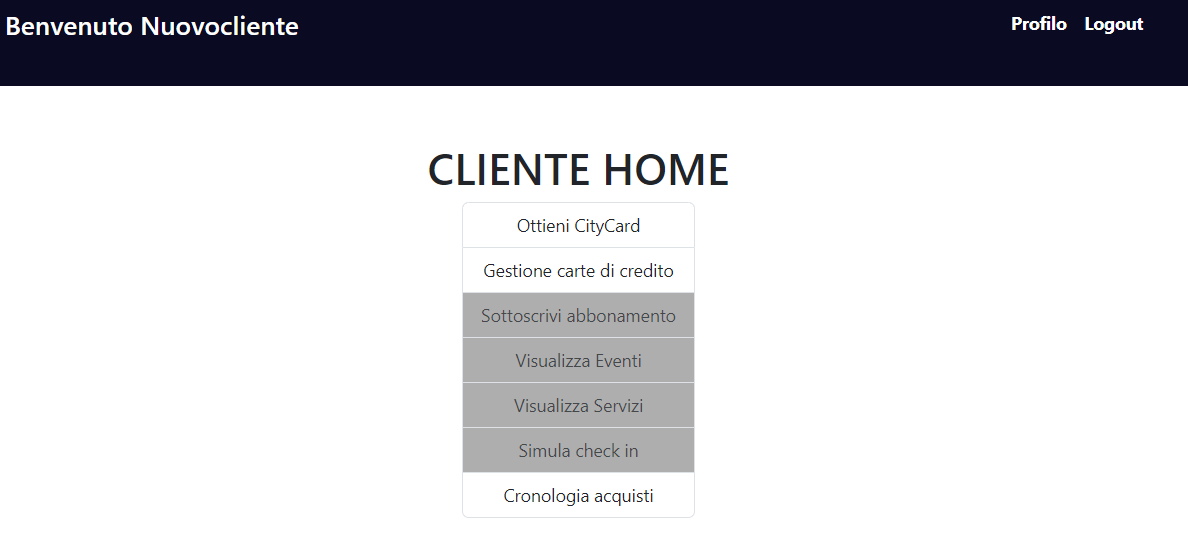
\includegraphics[width=0.95\columnwidth]{cliente_home_1.png}}
\end{center}
Al primo login login il cliente avrà disabilitate gran parte delle funzionalità in quanto non ancora in possesso di una CityCard e di un abbonamento attivo.
\begin{itemize}
    \item Ottieni CityCard
    \item Gestione carte di credito
    \item Cronologia acquisti
\end{itemize}
\begin{center}
    \fbox{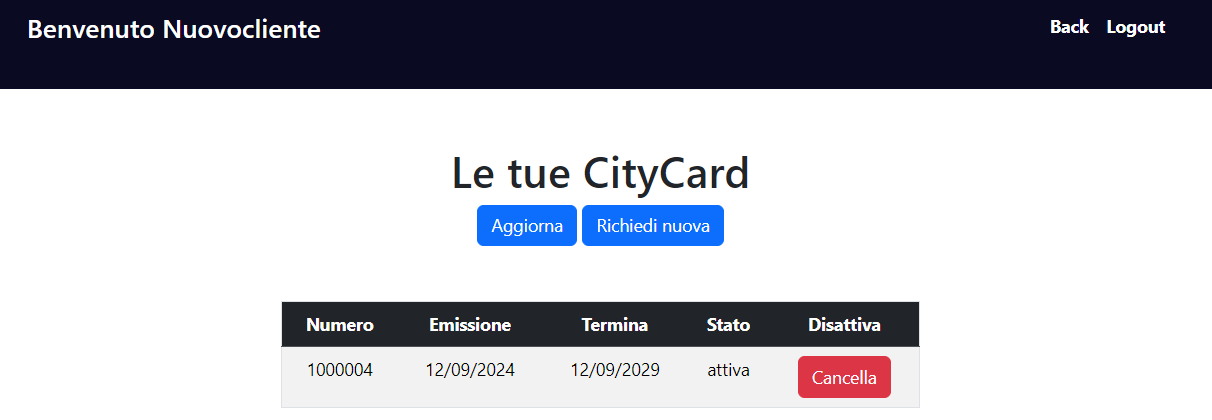
\includegraphics[width=0.95\columnwidth]{cliente_citycard.png}}
\end{center}
\begin{center}
    \fbox{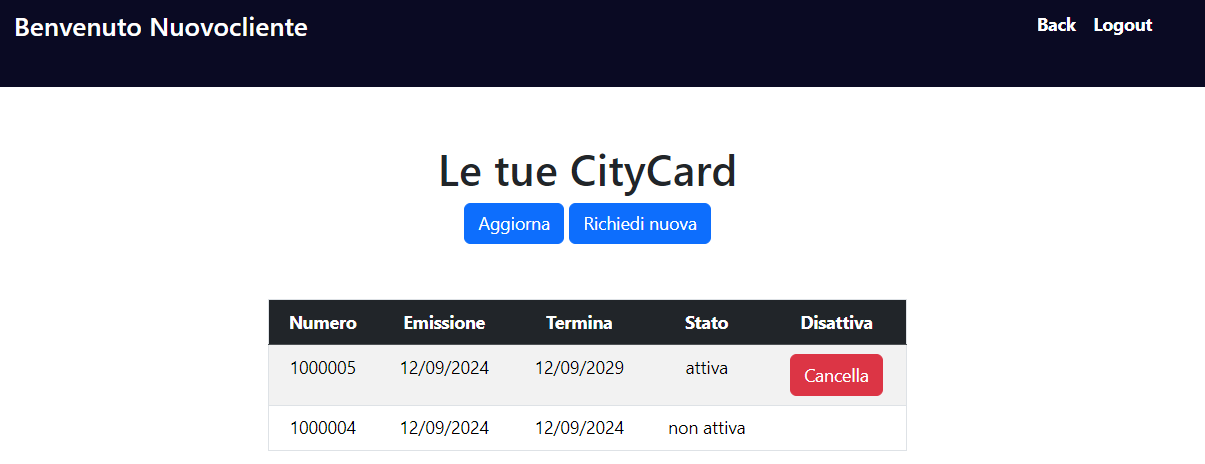
\includegraphics[width=0.95\columnwidth]{cliente_citycard_2.png}}
\end{center}
Il cliente può richiedere gratuitamente una nuova CityCard in qualsiasi momento, in caso di una ci fosse già una card attiva, questa verrà disattivata e ne verrà creata una nuova.
\begin{center}
    \fbox{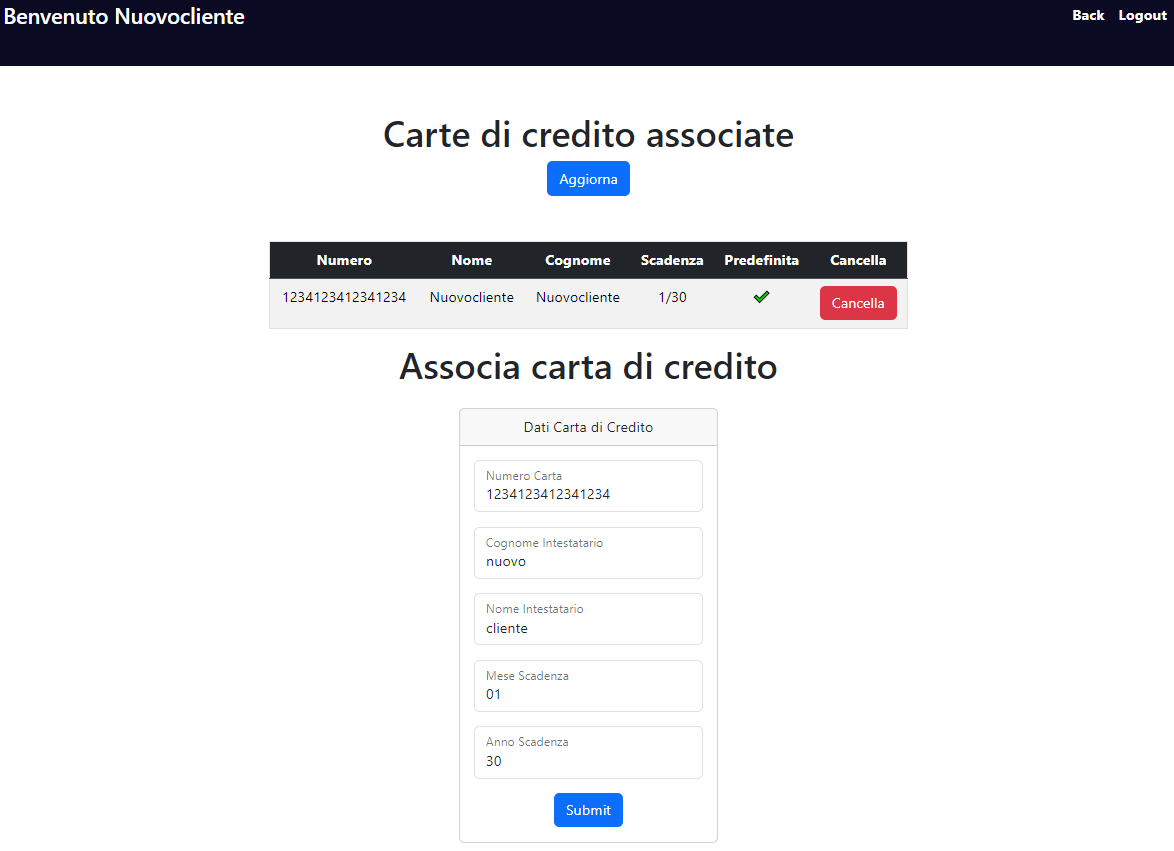
\includegraphics[width=0.95\columnwidth]{cliente_creditcard.png}}
\end{center}
In questa sezione il cliente può aggiungere le sue carte di credito e renderne predefinita una tra queste.
\begin{center}
    \fbox{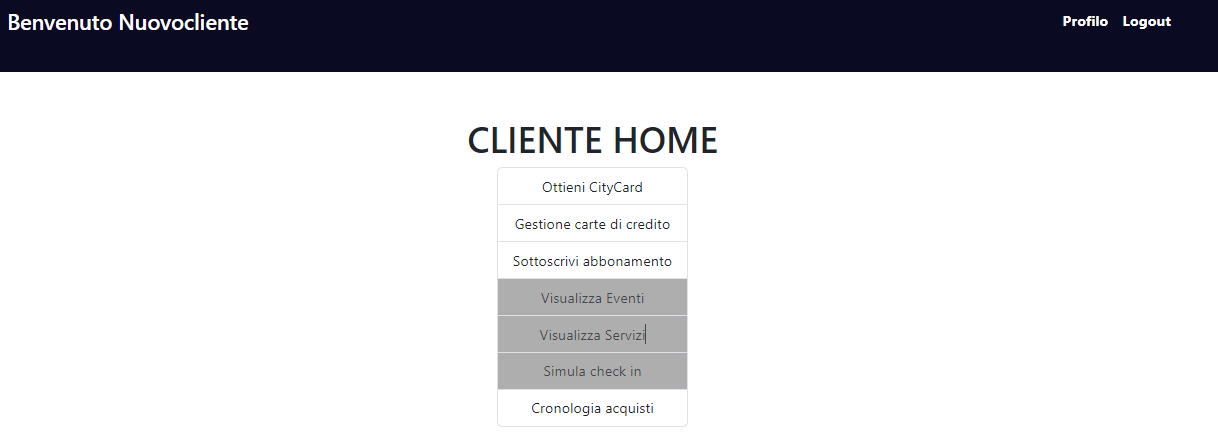
\includegraphics[width=0.95\columnwidth]{cliente_home_2.png}}
\end{center}
Una volta acquisita una CityCard e aggiunta una carta di credito predefinita verrà sbloccata nel menù la possibilità di sottoscrivere un abbonamento.
\begin{center}
    \fbox{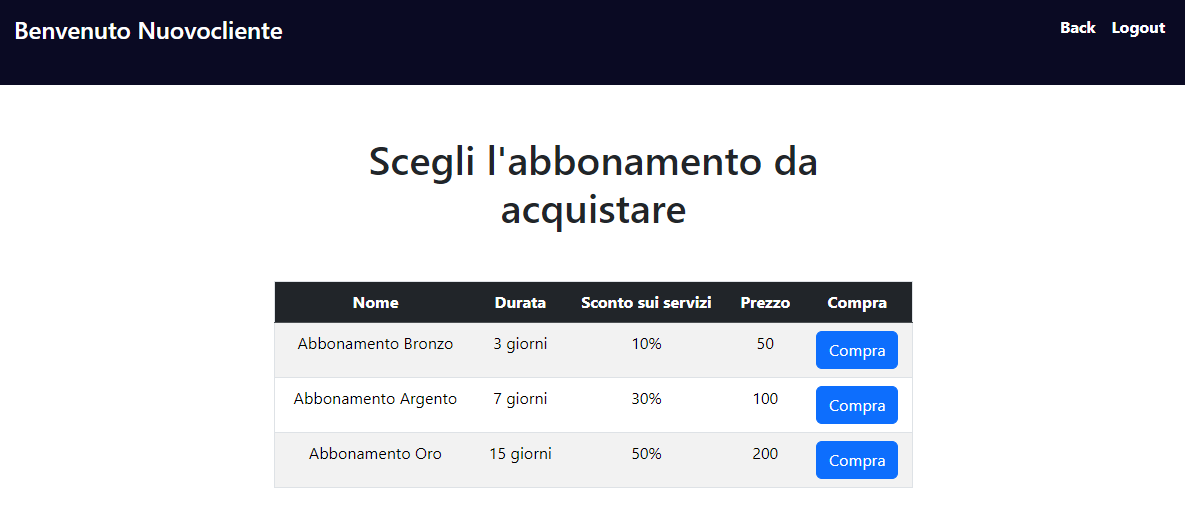
\includegraphics[width=0.95\columnwidth]{cliente_abbonamento.png}}
\end{center}
Una volta ottenuta la tessera sarà disponibile la sezione "Acquista abbonamento" dove sarà possibile scegliere tra tre tipologie di sottoscrizione.
\begin{center}
    \fbox{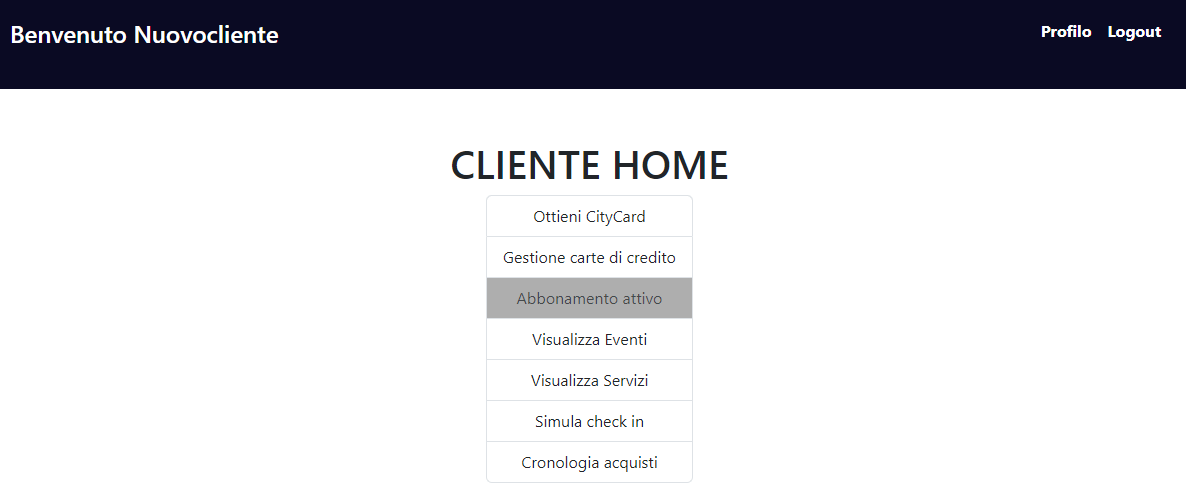
\includegraphics[width=0.95\columnwidth]{cliente_home_3.png}}
\end{center}
Dopo aver sottoscritto un abbonamento anche il resto del menù sarà sbloccato e sarà possibile, accetto la sezione per sottoscrivere abbonamenti.
\begin{itemize}
    \item Ottieni CityCard
    \item Gestione carte di credito
    \item Visualizza eventi
    \item Visualizza servizi
    \item Simula check in
    \item Cronologia acquisti
\end{itemize}
\begin{center}
    \fbox{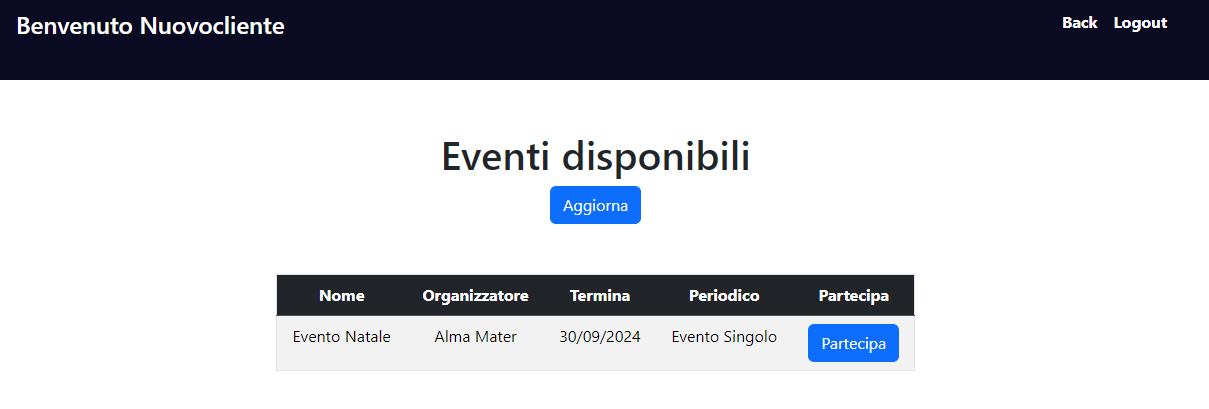
\includegraphics[width=0.95\columnwidth]{cliente_eventi.png}}
\end{center}
\begin{center}
    \fbox{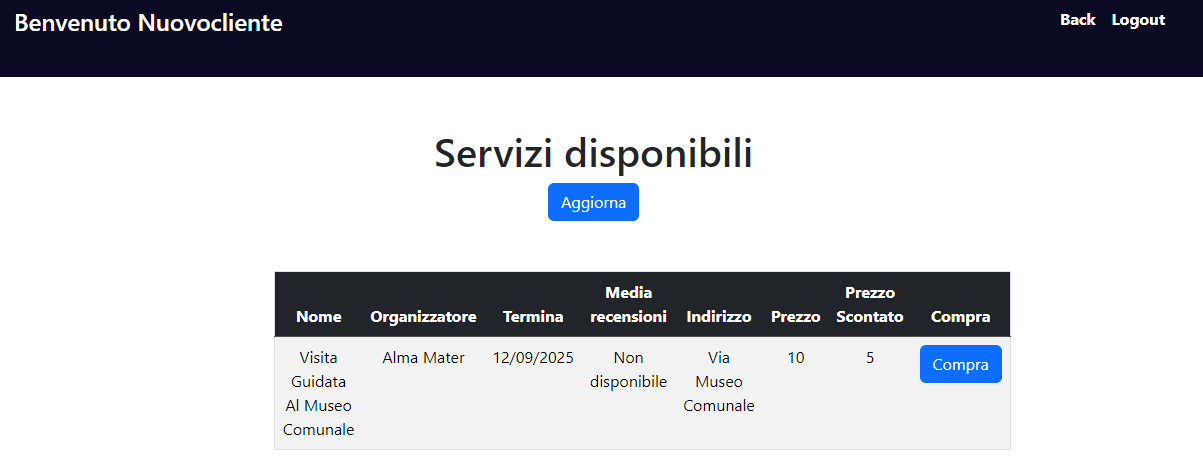
\includegraphics[width=0.95\columnwidth]{cliente_servizi.png}}
\end{center}
Il cliente può visualizzare e acquistare servizi o prenotare eventi.
\begin{center}
    \fbox{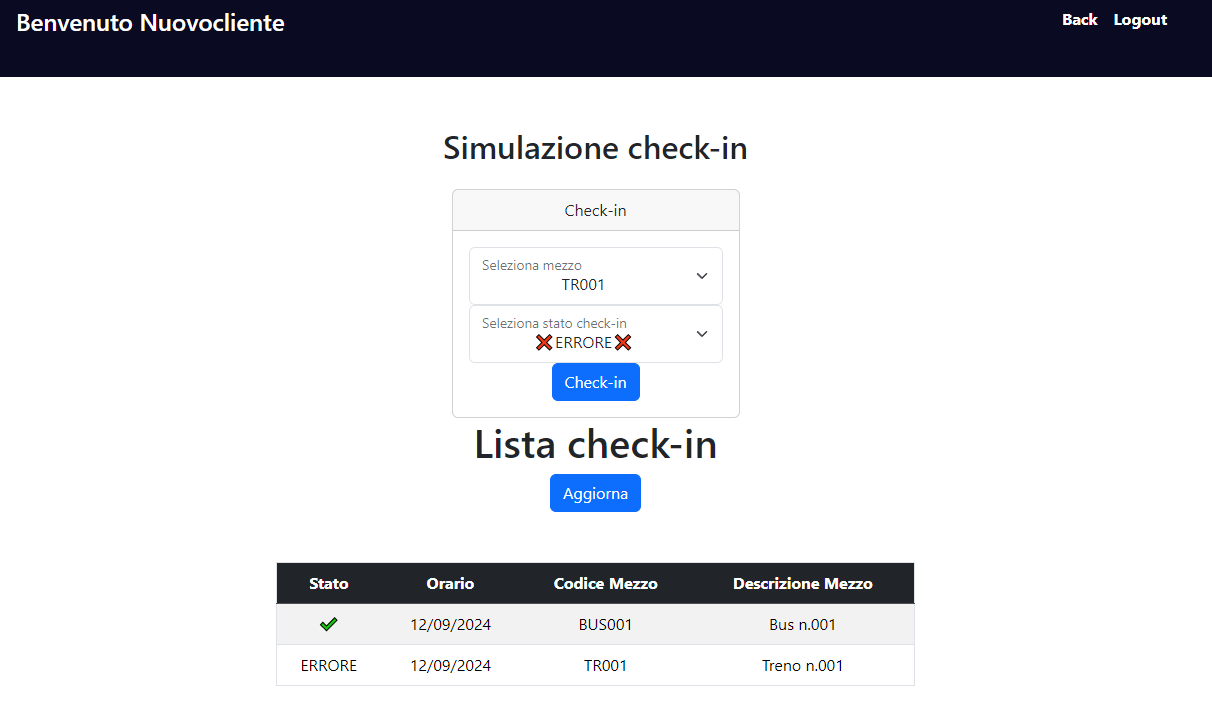
\includegraphics[width=0.95\columnwidth]{cliente_checkin.png}}
\end{center}
In questa sezione sarà possibile accedere al simulatore di checkin per l'utilizzo del dei trasporti pubblici.
\begin{center}
    \fbox{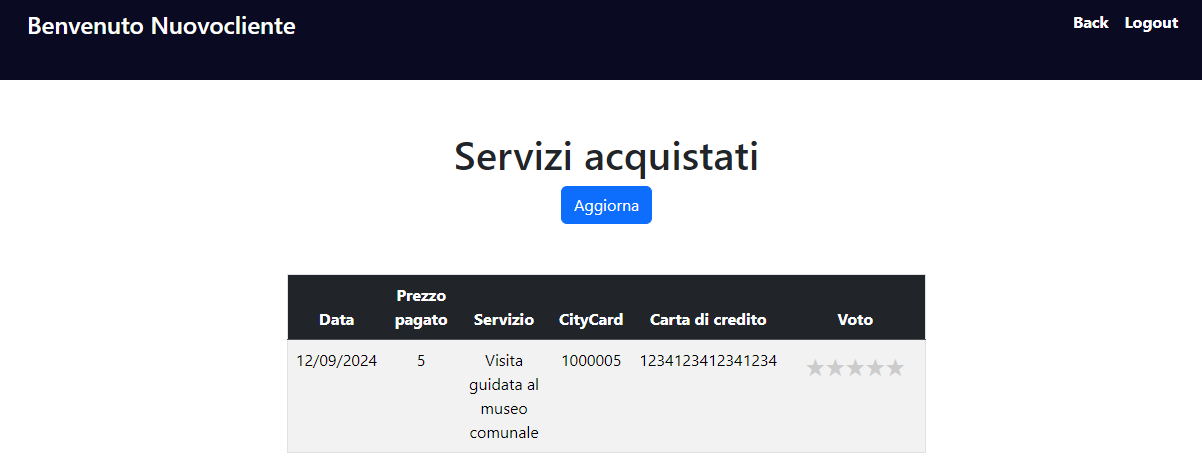
\includegraphics[width=0.95\columnwidth]{cliente_acquisti.png}}
\end{center}
Il cliente può visualizzare la cronologia degli acquisti fatti e dare un voto a ciascuno.

